\section{Decision Tree (Revisited) [9 pts]}


\begin{enumerate}

    \item \textbf{[2pt]} Suppose you are the 10-601 instructor trying to predict students' final exam grade using only homework grades. You decide to use historic records on this course to build a predictive model. However, someone messed up CMU's academic records system and the only information you have on students from past semesters is (i) if a student has submitted all homework (ii) if a student has attained maximum score on any of the homework (iii) if a student has scored 0 on any of the homework and  (iv) the students' letter grades on their final exams (this is the target, not attribute). You decide to use Decision Tree model, and since the information is so limited, you are satisfied as long as your model can predict the letter grade on the final exams  (A+, A, A-, B+, B, B-, C+, C and C-). Suppose that you have designed the grading policy to be percentile-based so all letter grades will show up. \\ \\
    Given enough past records and enough luck, will your model be able to do a perfect job (i.e., make no mistakes on students' letter grades of current semester)?
    
    \begin{list}{}
        \item $\circle$ Yes
        \item $\blackcircle$ No
    \end{list}
    Why or why not? Explain your reason briefly (you can use mathematical expressions).\\
    
    \textbf{NOTE: Please do not change the size of the following text box, and keep your answer in it. Thank you!} \\ \\
    \begin{tcolorbox}[fit,height=2cm, width=15cm, blank, borderline={1pt}{-2pt},nobeforeafter]
    \large
    The number of classes(9) is much larger than the number of attributes(3) so our model cannot make accurate predictions. The leaf nodes aren't enough to predict all classes.

    \end{tcolorbox} \\
    
    \newpage
    \item \textbf{[2pt]} Consider the following $4\times 4$ checkerboard pattern. 
    \begin{figure}[H]
        \centering
        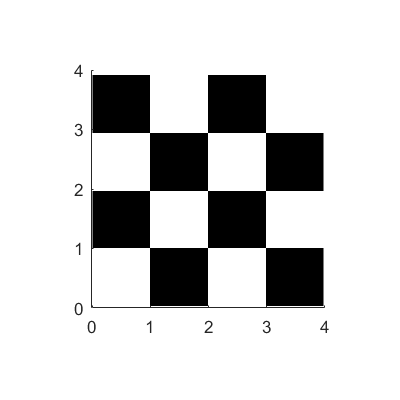
\includegraphics[width = 0.5\textwidth]{checkerboard.png}
        \label{Q_2dt}
    \end{figure}
    \begin{enumerate}
        \item What is the minimum depth of decision tree that perfectly classifies the $4\times 4$ colored regions, using $x$ and $y$ coordinates as separate features (how you use each of them is up to you)?
    \begin{list}{}
        \item $\circle$ 1
        \item $\blackcircle$ 2
        \item $\circle$ 4
        \item $\circle$ 16
    \end{list}
    \item What is the minimum depth of decision trees to perfectly classify the colored regions, using ANY features?
    \begin{list}{}
        \item $\blackcircle$ 1
        \item $\circle$ 2
        \item $\circle$ 4
        \item $\circle$ 16
    \end{list}
    \end{enumerate}
    
    \item \textbf{[3pt] Ensemble of Decision Tree.} Say we have a data set shown below. In total, there are 12 data points, with 6 in label "-" and 6 in label "+". We would like to use Decision Tree to solve this binary classification problem. However, in our problem setting, each Decision Tree has access to only ONE line. That is to say, our Decision Tree would have access to only one attribute, and so has max-depth of 1. \\ \\
    By accessing this line, the Decision Tree could know (and only know) whether the data point is on the right side of this line or the left side. (Unofficial definition: let's assume the right side of a line shares the same direction with the \textcolor{OliveGreen}{\textbf{green}} normal vector of that line.) \\ \\
    Finally, please use majority vote strategy to make classification decision at each leaf.\\
    
    \begin{figure}[H]
        \centering
        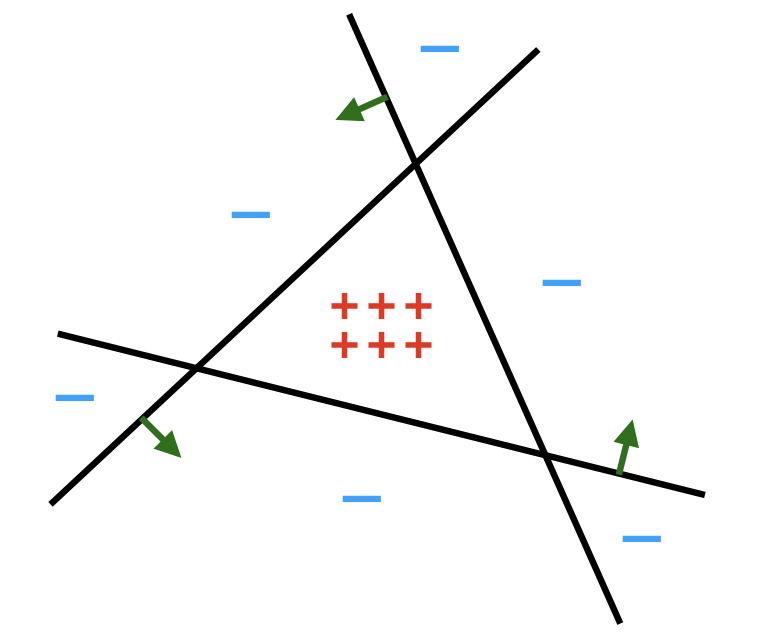
\includegraphics[width = 0.5\textwidth]{ensemble_dt.png}
        \label{Q_ensemble_DT}
    \end{figure}
    
    \begin{enumerate}
        \item  If we train only one Decision Tree, what is the best/lowest error rate? Note that we have in total 12 data points. (Please round to 4 decimal.) \\ \\
    \begin{tcolorbox}[fit,height=1cm, width=15cm, blank, borderline={1pt}{-2pt}, nobeforeafter]
    %solution
    \begin{center}\huge0.2500\end{center}
    \end{tcolorbox} 
    
    

    \item If we could use two Decision Trees, what is the best/lowest error rate? Let's say, if we have two Decision Trees, then each would predict each data point with label like '+' or '-'. Then we would like to combine these predictions as the final result. If these two all predict '+', then the result is '+'. The same with '-'. However, if one predicts '+' while one predicts '-', then to break tie, we always choose '-' as the final result. (Please round to 4 decimal.) \\ \\
    \begin{tcolorbox}[fit,height=1cm, width=15cm, blank, borderline={1pt}{-2pt}, nobeforeafter]
    %solution
    \begin{center}\huge0.0833\end{center}
    \end{tcolorbox} \\
    
    

\newpage
    \item Now let's train three Decision Trees as a forest, what is the best/lowest error rate? The ensemble strategy is now unanimous voting. That is, if every Decision Tree agree, then the final result is positive. However, if one of them has a different answer from the other two, then we predict negative. That means, we train each DT individually, with each DT choose one unique line as its decision boundary. Each DT would try its best to achieve high accuracy. And, next, if all DTs agrees, then it will give positive label. (Please round to 4 decimal.) \\ \\
    \begin{tcolorbox}[fit,height=1cm, width=15cm, blank, borderline={1pt}{-2pt}, nobeforeafter]
    %solution
    \begin{center}\huge0.0000\end{center}
    \end{tcolorbox} \\
    
    \end{enumerate}
    
    \item \textbf{[2pt]} Consider a binary classification problem using $1$-nearest neighbors. We have $N$ 1-dimensional training points $x_1, x_2, \ldots x_N$ and corresponding labels $y_1, y_2, \ldots y_N$ with $x_i \in \mathbb{R}$ and $y_i \in \{0, 1\}$. Assume the points $x_1, x_2, \ldots x_N$ are in ascending order by value. If there are ties during the 1-NN algorithm, we break ties by choosing the label of the $x_i$ with lower value. Assume we are using the Euclidean distance metric. Is it possible to build a decision tree where the decision at each node takes the form of “$x \leq t$ or $x > t$”, where $t \in \mathbb{R}$ behaves exactly the same as the 1-nearest neighbor classifier?
    
    \begin{list}{}
        \item $\blackcircle$ Yes
        \item $\circle$ No
    \end{list}
     If your answer is yes, please explain how you will construct the decision tree. If your answer is no, explain why it’s not possible.  \\
   
    \textbf{NOTE: Please do not change the size of the following text box, and keep your answer in it. Thank you!} \\ \\
    \begin{tcolorbox}[fit,height=4cm, width=15cm, blank, borderline={1pt}{-2pt},nobeforeafter]
    \large
    Let $x$ a point whose label we want to predict. If $x \leq \frac{x_1+x_2}{2}$, then predict $y_1$, otherwise keep splitting and check if $x \leq \frac{x_2+x_3}{2}$. If, this is true, predict $y_2$. Repeat the same process and eventually $x$ will be correctly classified.

    \end{tcolorbox} \\
    
    

    

\end{enumerate}



